% A simple graph with straight and bend arrows and loops
% Stefan Kottwitz
\documentclass{article}
\usepackage{tikz}
\usepackage{multirow}
\newcommand{\8}{$\infty$}
\newcommand{\ezA}{\begin{tabular}{|c|c|c|c|c|c|}
\hline\multicolumn{2}{|c|}{\multirow{2}{*}{$\mathrm{D}^\mathrm{A}$}} & \multicolumn{4}{|c|}{Cost via}\\ \cline{3-6}\multicolumn{2}{|c|}{}& B & C & D & E\\ \hline\multirow{4}{*}{\rotatebox{90}{Destination}}}

\newcommand{\ezB}{\begin{tabular}{|c|c|c|c|c|c|}
\hline\multicolumn{2}{|c|}{\multirow{2}{*}{$\mathrm{D}^\mathrm{B}$}} & \multicolumn{4}{|c|}{Cost via}\\ \cline{3-6}\multicolumn{2}{|c|}{}& A & C & D & E\\ \hline\multirow{4}{*}{\rotatebox{90}{Destination}}}

\newcommand{\ezC}{\begin{tabular}{|c|c|c|c|c|c|}
\hline\multicolumn{2}{|c|}{\multirow{2}{*}{$\mathrm{D}^\mathrm{C}$}} & \multicolumn{4}{|c|}{Cost via}\\ \cline{3-6}\multicolumn{2}{|c|}{}& A & B & D & E\\ \hline\multirow{4}{*}{\rotatebox{90}{Destination}}}

\newcommand{\ezD}{\begin{tabular}{|c|c|c|c|c|c|}
\hline\multicolumn{2}{|c|}{\multirow{2}{*}{$\mathrm{D}^\mathrm{D}$}} & \multicolumn{4}{|c|}{Cost via}\\ \cline{3-6}\multicolumn{2}{|c|}{}& A & B & C & E\\ \hline\multirow{4}{*}{\rotatebox{90}{Destination}}}

\newcommand{\ezE}{\begin{tabular}{|c|c|c|c|c|c|}
\hline\multicolumn{2}{|c|}{\multirow{2}{*}{$\mathrm{D}^\mathrm{E}$}} & \multicolumn{4}{|c|}{Cost via}\\ \cline{3-6}\multicolumn{2}{|c|}{}& A & B & C & D\\ \hline\multirow{4}{*}{\rotatebox{90}{Destination}}}

\newcommand{\ze}{\end{tabular}}

\newcommand{\upd}{\begin{tabular}{c|c}}

\begin{document}

\section{3.1}
\subsection{3.1.1}
%%% 3.1.1. %%%
The Graph:\\
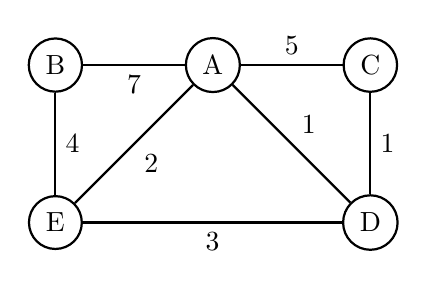
\begin{tikzpicture}[-,
					%>=stealth',
					%shorten >=1pt,
					auto,
					node distance=2cm,
					thick,
					main node/.style={circle,draw}]

  \node[main node] (A) {A};
  \node[main node] (B) [left of=A] {B};
  \node[main node] (C) [right of=A] {C};
  \node[main node] (D) [below of=C] {D};
  \node[main node] (E) [below of=B] {E};
  
  \path[every node/.style={}]
    (A) edge node {7} (B)
        edge node {5} (C)
        edge node {1} (D)
        edge node {2} (E)
    (B) edge node {4} (E)
  	(C) edge node {1} (D)
  	(D) edge node {3} (E);
\end{tikzpicture}
\\
Distance Tables after Initialisation Phase:
\\
\begin{tabular}{c|c|c}
Destination & Cost & Via \\ \hline
B           & 7    & B   \\
C           & 5    & C   \\
D           & 1    & D   \\
E           & 2    & E   \\
\end{tabular}
\begin{tabular}{c|c|c}
Destination & Cost & Via \\ \hline
A           & 7    & A   \\
C           &      &     \\
D           &      &     \\
E           & 4    & E   \\
\end{tabular}
\begin{tabular}{c|c|c}
Destination & Cost & Via \\ \hline
A           & 5    & A   \\
B           &      &     \\
D           & 1    & D   \\
E           &      &     \\
\end{tabular}
\begin{tabular}{c|c|c}
Destination & Cost & Via \\ \hline
A           & 1    & A   \\
B           &      &     \\
C           & 1    & C   \\
E           & 3    & E   \\
\end{tabular}
\begin{tabular}{c|c|c}
Destination & Cost & Via \\ \hline
A           & 2    & A   \\
B           & 4    & B   \\
C           &      &     \\
D           & 3    & D   \\
\end{tabular}

The first update messages:\\
\begin{tabular}{|c|c|@{}c@{}|@{}c@{}|@{}c@{}|@{}c@{}|@{}c@{}|}
\hline \multicolumn{2}{|c|}{Update} & \multicolumn{5}{|c|}{sent to:} \\ \cline{3-7} \multicolumn{2}{|c|}{Messages} & A & B & C & D & E \\ \hline \multirow{5}{*}{\rotatebox{90}{sent by:}}
& A & &
\upd
to C & 5 \\ to D & 1 \\ to E & 2 \\
\end{tabular} &
\upd
to B & 7 \\ to D & 1 \\ to E & 2 \\
\end{tabular} &
\upd
to B & 7 \\ to C & 5 \\ to E & 2 \\
\end{tabular} &
\upd
to B & 7 \\ to C & 5 \\ to D & 1 \\
\end{tabular} \\ \cline{2-7}
& B &
\upd
to E & 4 \\
\end{tabular} & & & &
\upd
to A & 7 \\
\end{tabular} \\ \cline{2-7}
& C &
\upd
to D & 1
\end{tabular} & & &
\upd
to A & 5
\end{tabular} & \\ \cline{2-7}
& D &
\upd
to C & 1 \\ to E & 3 \\
\end{tabular} & &
\upd
to A & 1 \\ to E & 3 \\
\end{tabular} & &
\upd
to A & 1 \\ to C & 1 \\
\end{tabular} \\ \cline{2-7}
& E &
\upd
to B & 4 \\ to D & 3 \\
\end{tabular} &
\upd
to A & 2 \\ to D & 3 \\
\end{tabular} & &
\upd
to A & 2 \\ to B & 4 \\
\end{tabular} &
\\ \hline
\end{tabular}


\clearpage
%%% 3.1.2 %%%
\subsection{3.1.2}
Distance Tables Iteration 1:\\
\begin{tabular}{c|c|c}
Destination & Cost & Via \\ \hline
B           & 6    & E   \\
C           & 2    & D   \\
D           & 1    & D   \\
E           & 2    & E   \\
\end{tabular}
\begin{tabular}{c|c|c}
Destination & Cost & Via \\ \hline
A           & 6    & A   \\
C           & 11   & E   \\
D           & 7    & E   \\
E           & 4    & E   \\
\end{tabular}
\begin{tabular}{c|c|c}
Destination & Cost & Via \\ \hline
A           & 2    & D   \\
B           & 9    & D   \\
D           & 1    & D   \\
E           & 4    & D   \\
\end{tabular}
\begin{tabular}{c|c|c}
Destination & Cost & Via \\ \hline
A           & 1    & A   \\
B           & 7    & E   \\
C           & 1    & C   \\
E           & 3    & E   \\
\end{tabular}
\begin{tabular}{c|c|c}
Destination & Cost & Via \\ \hline
A           & 2    & A   \\
B           & 4    & B   \\
C           & 4    & D   \\
D           & 3    & D   \\
\end{tabular}
\\
Update Messages Iteration 1:\\
\begin{tabular}{|c|c|@{}c@{}|@{}c@{}|@{}c@{}|@{}c@{}|@{}c@{}|}
\hline \multicolumn{2}{|c|}{Update} & \multicolumn{5}{|c|}{sent to:} \\ \cline{3-7} \multicolumn{2}{|c|}{Messages} & A & B & C & D & E \\ \hline \multirow{5}{*}{\rotatebox{90}{sent by:}}
&A&&
\upd      &   \\ to C & 2\ze &
\upd to B & 6 \\      &  \ze &
\upd to B & 6 \\ to C & 2\ze &
\upd to B & 6 \\ to C & 2\ze \\ \cline{2-7}
&B&
\upd to C & 11 \\ to D & 7 \ze &&&&
\upd to C & 11 \\ to D & 7 \ze \\ \cline{2-7}
&C&
\upd      &   \\ to B & 9 \\ to E & 4\ze &&&
\upd to A & 2 \\ to B & 9 \\ to E & 4\ze & \\ \cline{2-7}
&D&
\upd to B & 7\ze &&
\upd to B & 7\ze &&
\upd to B & 7\ze \\ \cline{2-7}
&E&
\upd to C & 4\ze &
\upd to C & 4\ze &
\upd \ze &
\upd to C & 4\ze &\\ \hline
\end{tabular}\\
%\clearpage
Distance Tables Iteration 2:\\
\begin{tabular}{c|c|c}
Destination & Cost & Via \\ \hline
B           & 6    & E   \\
C           & 2    & D   \\
D           & 1    & D   \\
E           & 2    & E   \\
\end{tabular}
\begin{tabular}{c|c|c}
Destination & Cost & Via \\ \hline
A           & 6    & A   \\
C           & 8    & A   \\
D           & 7    & E   \\
E           & 4    & E   \\
\end{tabular}
\begin{tabular}{c|c|c}
Destination & Cost & Via \\ \hline
A           & 2    & D   \\
B           & 8    & D   \\
D           & 1    & D   \\
E           & 4    & D   \\
\end{tabular}
\begin{tabular}{c|c|c}
Destination & Cost & Via \\ \hline
A           & 1    & A   \\
B           & 7    & E   \\
C           & 1    & C   \\
E           & 3    & E   \\
\end{tabular}
\begin{tabular}{c|c|c}
Destination & Cost & Via \\ \hline
A           & 2    & A   \\
B           & 4    & B   \\
C           & 4    & D   \\
D           & 3    & D   \\
\end{tabular}
\\
Update Messages Iteration 2:\\
\begin{tabular}{|c|c|@{}c@{}|@{}c@{}|@{}c@{}|@{}c@{}|@{}c@{}|}
\hline \multicolumn{2}{|c|}{Update} & \multicolumn{5}{|c|}{sent to:} \\ \cline{3-7} \multicolumn{2}{|c|}{Messages} & A & B & C & D & E \\ \hline \multirow{5}{*}{\rotatebox{90}{sent by:}}
&A&&&&&\\ \cline{2-7}
&B&\upd to C & 8\ze &&&\upd to C & 8\ze &\\ \cline{2-7}
&C&\upd to B & 8\ze &&&\upd to B & 8\ze &\\ \cline{2-7}
&D&&&&&\\ \cline{2-7}
&E&&&&&\\ \hline
\end{tabular}

After the second iteration, no more update messages are sent.
\clearpage
\subsection{3.1.3}
The Graph:\\
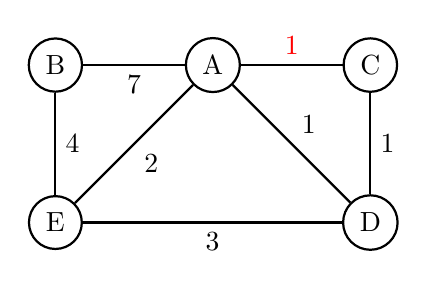
\begin{tikzpicture}[-,
					%>=stealth',
					%shorten >=1pt,
					auto,
					node distance=2cm,
					thick,
					main node/.style={circle,draw}]

  \node[main node] (A) {A};
  \node[main node] (B) [left of=A] {B};
  \node[main node] (C) [right of=A] {C};
  \node[main node] (D) [below of=C] {D};
  \node[main node] (E) [below of=B] {E};
  
  \path[every node/.style={}]
    (A) edge node {7} (B)
        edge node {\textcolor{red}{1}} (C)
        edge node {1} (D)
        edge node {2} (E)
    (B) edge node {4} (E)
  	(C) edge node {1} (D)
  	(D) edge node {3} (E);
\end{tikzpicture}
\\
Distance Tables after Initialisation Phase:
\\
\begin{tabular}{c|c|c}
Destination & Cost & Via \\ \hline
B           & 7    & B   \\
C           & \textcolor{red}{1}    & C   \\
D           & 1    & D   \\
E           & 2    & E   \\
\end{tabular}
\begin{tabular}{c|c|c}
Destination & Cost & Via \\ \hline
A           & 7    & A   \\
C           &      &     \\
D           &      &     \\
E           & 4    & E   \\
\end{tabular}
\begin{tabular}{c|c|c}
Destination & Cost & Via \\ \hline
A           & \textcolor{red}{1}    & A   \\
B           &      &     \\
D           & 1    & D   \\
E           &      &     \\
\end{tabular}
\begin{tabular}{c|c|c}
Destination & Cost & Via \\ \hline
A           & 1    & A   \\
B           &      &     \\
C           & 1    & C   \\
E           & 3    & E   \\
\end{tabular}
\begin{tabular}{c|c|c}
Destination & Cost & Via \\ \hline
A           & 2    & A   \\
B           & 4    & B   \\
C           &      &     \\
D           & 3    & D   \\
\end{tabular}
\\The first update messages:\\
\begin{tabular}{|c|c|@{}c@{}|@{}c@{}|@{}c@{}|@{}c@{}|@{}c@{}|}
\hline \multicolumn{2}{|c|}{Update} & \multicolumn{5}{|c|}{sent to:} \\ \cline{3-7} \multicolumn{2}{|c|}{Messages} & A & B & C & D & E \\ \hline \multirow{5}{*}{\rotatebox{90}{sent by:}}
& A & &
\upd
to C & \textcolor{red}{1} \\ to D & 1 \\ to E & 2 \\
\end{tabular} &
\upd
to B & 7 \\ to D & 1 \\ to E & 2 \\
\end{tabular} &
\upd
to B & 7 \\ to C & \textcolor{red}{1} \\ to E & 2 \\
\end{tabular} &
\upd
to B & 7 \\ to C & \textcolor{red}{1} \\ to D & 1 \\
\end{tabular} \\ \cline{2-7}
& B &
\upd
to E & 4 \\
\end{tabular} & & & &
\upd
to A & 7 \\
\end{tabular} \\ \cline{2-7}
& C &
\upd
to D & 1
\end{tabular} & & &
\upd
to A & \textcolor{red}{1}
\end{tabular} & \\ \cline{2-7}
& D &
\upd
to C & 1 \\ to E & 3 \\
\end{tabular} & &
\upd
to A & 1 \\ to E & 3 \\
\end{tabular} & &
\upd
to A & 1 \\ to C & 1 \\
\end{tabular} \\ \cline{2-7}
& E &
\upd
to B & 4 \\ to D & 3 \\
\end{tabular} &
\upd
to A & 2 \\ to D & 3 \\
\end{tabular} & &
\upd
to A & 2 \\ to B & 4 \\
\end{tabular} &
\\ \hline
\end{tabular}
\\Distance Tables Iteration 1:\\
\begin{tabular}{c|c|c}
Destination & Cost & Via \\ \hline
B           & 6    & E   \\
C           & \textcolor{red}{1}    & \textcolor{red}{C}   \\
D           & 1    & D   \\
E           & 2    & E   \\
\end{tabular}
\begin{tabular}{c|c|c}
Destination & Cost & Via \\ \hline
A           & 6    & A   \\
C           & \textcolor{red}{8}   & \textcolor{red}{E}   \\
D           & 7    & E   \\
E           & 4    & E   \\
\end{tabular}
\begin{tabular}{c|c|c}
Destination & Cost & Via \\ \hline
A           & \textcolor{red}{1}    & \textcolor{red}{A}   \\
B           & \textcolor{red}{8}    & \textcolor{red}{A}   \\
D           & 1    & D   \\
E           & \textcolor{red}{3}    & \textcolor{red}{A}   \\
\end{tabular}
\begin{tabular}{c|c|c}
Destination & Cost & Via \\ \hline
A           & 1    & A   \\
B           & 7    & E   \\
C           & 1    & C   \\
E           & 3    & E   \\
\end{tabular}
\begin{tabular}{c|c|c}
Destination & Cost & Via \\ \hline
A           & 2    & A   \\
B           & 4    & B   \\
C           & \textcolor{red}{3}    & \textcolor{red}{A}   \\
D           & 3    & D   \\
\end{tabular}
\\
Update Messages Iteration 1:\\
\begin{tabular}{|c|c|@{}c@{}|@{}c@{}|@{}c@{}|@{}c@{}|@{}c@{}|}
\hline \multicolumn{2}{|c|}{Update} & \multicolumn{5}{|c|}{sent to:} \\ \cline{3-7} \multicolumn{2}{|c|}{Messages} & A & B & C & D & E \\ \hline \multirow{5}{*}{\rotatebox{90}{sent by:}}
&A&&
\upd      &   \\ \colorbox{red}{\textcolor{red}{to C}} & \colorbox{red}{\textcolor{red}{2}}\ze &
\upd to B & 6 \\      &  \ze &
\upd to B & 6 \\ \colorbox{red}{\textcolor{red}{to C}} & \colorbox{red}{\textcolor{red}{2}}\ze &
\upd to B & 6 \\ \colorbox{red}{\textcolor{red}{to C}} & \colorbox{red}{\textcolor{red}{2}}\ze \\ \cline{2-7}
&B&
\upd to C & \textcolor{red}{8} \\ to D & 7 \ze &&&&
\upd to C  & \textcolor{red}{8} \\ to D & 7 \ze \\ \cline{2-7}
&C&
\upd      &   \\ to B & \textcolor{red}{8} \\ to E & \textcolor{red}{3}\ze &&&
\upd \colorbox{red}{\textcolor{red}{to A}} & \colorbox{red}{\textcolor{red}{2}} \\ to B & \textcolor{red}{8} \\ to E & \textcolor{red}{3}\ze & \\ \cline{2-7}
&D&
\upd to B & 7\ze &&
\upd to B & 7\ze &&
\upd to B & 7\ze \\ \cline{2-7}
&E&
\upd to C & \textcolor{red}{3}\ze &
\upd to C & \textcolor{red}{3}\ze &
\upd \ze &
\upd to C & \textcolor{red}{3}\ze &\\ \hline
\end{tabular}\\
After the first iteration, no more update messages are sent.

\subsection{3.1.4}
Wahrscheinlich will man hier hören, dass ein Count-To-Infinity eintritt - ich verstehe aber nicht, warum das so ist.
\colorbox{red}{\textcolor{white}{SOLUTION MISSING!}}
\subsection{3.1.5}
\colorbox{red}{\textcolor{white}{SOLUTION MISSING!}}
\subsection{3.1.6}
No it isn't. \colorbox{red}{\textcolor{white}{EXPLANATION HERE!}}
\end{document}
